\documentclass[10pt,a4paper]{article}
\usepackage[scale=0.75,a4paper]{geometry}
\usepackage[utf8]{inputenc}
\usepackage{amsmath}
\usepackage{amsfonts}
\usepackage{amssymb}
\usepackage{babel}
\usepackage{graphicx}




\author{Oduwole Eunice}
\title{Exploring Weather Trends}
\begin{document}
\maketitle

\section*{Data Extraction}
\noindent For this project, I considered  Finland (Helsinki), Spain (Madrid), Italy (Milan) to analyse the local temperature. The global data has 267 observation (1750 - 2015) and the three local afford mentioned cities has 268 (1743 - 2013). 

\noindent In order to extract data from the temperatures database, I ensure to verify if there were empty entries for both the global and local temperature  using the SQL command below:

\begin{list}{}{}
\item[1.] SELECT * FROM global$\_$data WHERE avg$\_$temp IS NULL 
\item[2.] SELECT year, city, country, avg$\_$temp FROM city$\_$data WHERE city = 'Helsinki' AND country = 'Finland' AND avg$\_$temp IS NULL
\item[3.] SELECT year, city, country, avg$\_$temp FROM city$\_$data WHERE city = 'Madrid' AND country = 'Spain' AND avg$\_$temp IS NULL
\item[4.] SELECT year, city, country, avg$\_$temp FROM city$\_$data WHERE city = 'Milan' AND country = 'Italy' AND avg$\_$temp IS NULL
\end{list}
There was no empty entries for the global data, however, for the local data there was four empty entries from 1746 to 1749. Thus, I omitted the empty entries and downloaded the data using the commands below respectively:  

\begin{list}{}{}
 \item[1.] SELECT * FROM global$\_$data 
 \item[2.] SELECT year, city, country, avg$\_$temp FROM city$\_$data WHERE city = 'Helsinki' AND country = 'Finland' AND avg$\_$temp IS NOT NULL
 \item[3.] SELECT year, city, country, avg$\_$temp FROM city$\_$data WHERE city = 'Madrid' AND country = 'Spain' AND avg$\_$temp IS NOT NULL
 \item[4.] SELECT year, city, country, avg$\_$temp FROM city$\_$data WHERE city = 'Milan' AND country = 'Italy' AND avg$\_$temp IS NOT NULL
\end{list}

\section*{Moving Average}
Ten years moving average was calculated using excel such that starting from the eleventh column /year, I calculate the average of the past ten years. Then, copied the cell and paste it all the way down to the end of the data. 

%\newpage

\section*{Correlation Coefficient}
I checked the correlation between the global data and the three local data from the result given in Table \ref{table1} below, it shows that there exist a strong positive relationship between them.

\begin{table}
\centering
\begin{tabular}{|c|c|}
\hline 
\multicolumn{2}{|c|}{Correlation} \\ 
\hline 
Helsinki & 0.8496 \\ 
\hline 
Italy & 0.8701 \\ 
\hline 
Spain & 0.8792 \\ 
\hline 
\end{tabular} 
\caption{Correlation table}
\label{table1}
\end{table}

\section*{Line chart and discussion}
Figure \ref{fig1} shows the line chart of global temperature in comparison to the three local temperature.

\begin{figure}[!h]
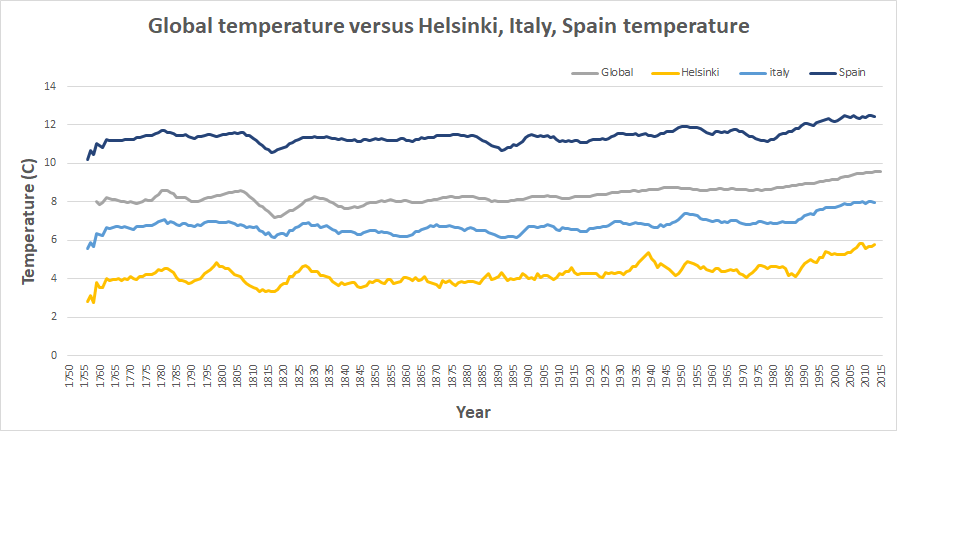
\includegraphics[scale=0.75]{Globaltemp.png} 
\caption{Global temperature in comparison with three local temperature}
\label{fig1}
\end{figure}

\noindent There appears to be similarity in the trend of the global temperature in comparison with the other two cities with Spain having a higher temperature and  following almost similar pattern. Between the year 1780 to 1796 there was a little drop in the temperature likewise with the global temperature. Between the year 1800 to 1825 there was also drop in Helsinki and Spain temperature, as well as global temperature. From 1835 to 1888 the temperature was almost stable with little fluctuations. The temperature appears to be growing hotter from 2000 to 2015 for the three local cities as also seen in the global temperature.

























\end{document}